\section{Friendly Dolphin}
  \subsection{Definición y objetivos}
    \paragraph{Éste módulo es el encargado de brindar la información procesada al usuario a través de una página de internet (véase Figura 8.1). Es el módo visual que los usuarios finales tendrán para poder interactuar con el ecosistema Ambienta2MX.}
    \paragraph{Se presenta cómo un módulo web que consumirá la información procesada y almacenada por las cuatro bases (MX1,MX2,MX3,MX4) y la base de soporte (Places).}
    \begin{figure}[h!]
        \centering
          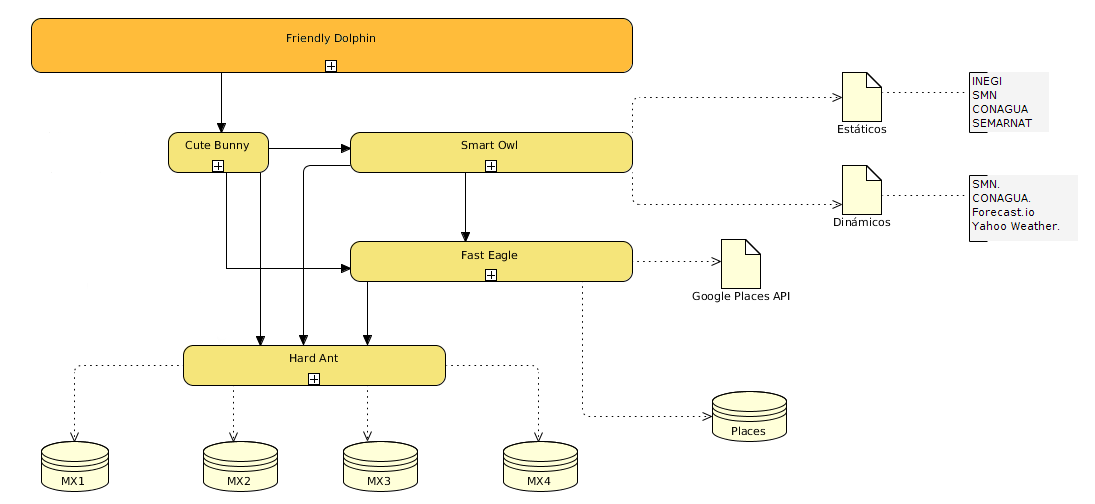
\includegraphics[width=\textwidth]{./images/DiagramaAmbienta2MX_FriendlyDolphin.png}
        \caption{Friendly Dolphin, Módulo de Ambienta2MX.}
    \end{figure}
    \paragraph{La principal función es la de consulta y visualización de datos. Es la capa más expuesta y visual de Ambienta2MX ya que es la que tendrá interacción directa con usuarios no técnicos, sin embargo, contará con los procesos necesarios para poder extraer información de las demás plataformas en formatos convencionales cómo JSON o CSV para uso posterior del usuario.}
  \subsection{Alcances}
    \paragraph{Interactúa de forma directa con el bloque \textbf{\emph{Cute Bunny}}, que forma parte de la segunda capa de exposición de datos de Ambienta2MX. Se comunica con los demás módulos mediante servicios de tipo REST que funcionan bajo el patrón de convención sobre configuración\cite{8}, brindando así una gran compatibilidad con éstos además de disminuir el tiempo de desarrollo debido a que no es necesario generar código único y se opta por la reutilización de éste además de apoyarse con el uso de bibliotecas que siguen el mismo método de trabajo.}
    \paragraph{Friendly Dolphin sólo puede ser visto como una herramienta de consulta, no podrá ser visto cómo un utensilio de análisis de datos climatológicos, es por ello que muestra la información en mapas, gráficas y detalles de la consulta.}
  \subsection{Restricciones}
    \paragraph{Éste módulo se ve limitado por la API de Google Maps para la visualización de la información, ya que las consultas resultan limitadas en su versión gratuita, sin embargo, la cantidad es suficiente para demostrar la aplicación de los datos en una herramienta de visualización. Las restricciones estan definidas a 25,000 solicitudes por día y limitada a un segundo por petición o usuario.}
    \paragraph{La vista también cuenta con cierta limitantes, sólo podrá ser visualizada en navegadores con Internet Explorer 11+, Mozilla Firefox 20+ y Google Chrome 20+}
  \subsection{Arquitectura}
    \paragraph{Friendly Dolpin contará con varios procesos y módulos a ser desarrollados (véase Figura 8.2). Éste módulo se desarrollará usando tecnologías cómo HTML, Javascript y CSS, además de contar con un ciclo continuo de desarrollo usando herramientas de apoyo cómo Yeoman, Gulp para el maquetado y gestión de tareas comunes en projectos de tipo web.}
    \paragraph{Se hará uso del servidor interno que ofrece Gulp junto con las tareas y gestión de bibliotecas de terceros. En cuanto al desarrollo de los estilos necesarios para las vistas se implementará Bootstrap cómo maquetado CSS y finalmente el manejo de vistas, peticiciones y lógica dentro del navegador de los clientes se implementará un patrón de tipo SPA (Single Page Application)\cite{36} desarrollado por el equipo de trabajo.}
    \begin{figure}[b!]
      \centering
        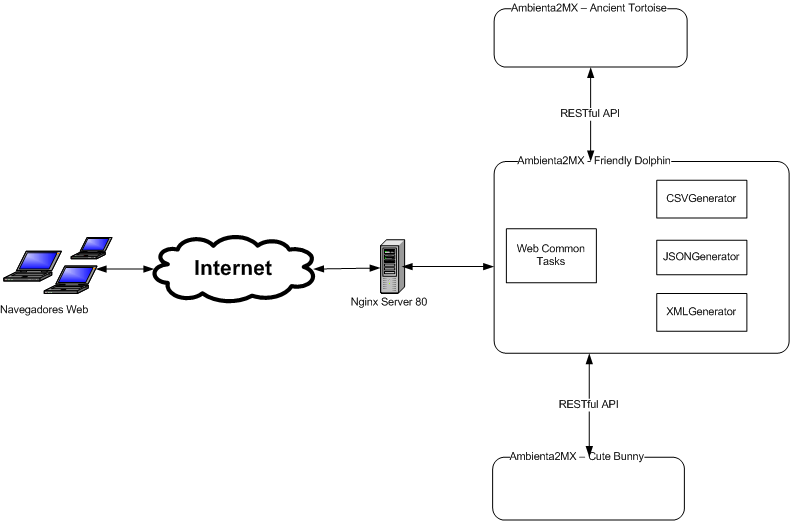
\includegraphics[width=\textwidth]{./images/DiagramaFriendlyDolphin.png}
      \caption{Diagrama General de Friendly Dolphin}
    \end{figure}
  \subsection{Factibilidad}   
    \paragraph{Se decidió cambiar de framework en las vistas, se quitó la implementación de EmberJs del proyecto y se optó por simplemente la ideología que éste tiene, considerando un patrón SPA\cite{36} mínimo ya que el framework antes mencionado contaba con demasiadas características que no iban a ser implementadas sin embargo el framework hace uso de estas.}
    \paragraph{Se optó por seguir esa ideología brindando la flexibilidad necesaria que consideró el equipo de trabajo para cumplir con el objetivo de tener una página dinámica que convive con los demás módulos de Ambienta2MX.}
    \paragraph{A continuación se muestran las características principales de cada tecnología:}
    \paragraph{``EmberJs''}    
    \begin{itemize}
      \item Manajo de un patrón SPA.
      \item Trabajo y desarrollo utilizando Convenció sobre configuración.
      \item Control de rutas, controladores, modelos, vistas, pruebas y dependencias externas.
      \item Implementación de plantillas (templates).
      \item Uso de AJAX como forma de interacción con servicios externos.
    \end{itemize}
    \paragraph{``Servicio Generado por el Equipo de Ambienta2MX''}    
    \begin{itemize}
      \item Uso de AJAX como forma de interacción con servicios externos.
      \item Manejo básico de templates para vistas.
      \item Control de rutas y datos adquiridos del servidor.
    \end{itemize}
    \paragraph{Cómo puede verse, el framework EmberJs contiene más caracteristicas que las necesarias para el desarrollo del proyecto, es por eso que decidió adaptarse esa misma ideología haciendo uso de  un framework mínimo creado por el equipo de Ambienta2MX totalmente adecuado a las necesidades que tiene en éste caso el módulo Friendly Dolphin.}
  \subsection{Pruebas y Capturas de pantalla}
    \paragraph{Para este módulo se realizaron pruebas funcionales indicando el flujo básico de información que un usuario común seguiría. Las pantallas básicas se muestran a continuación y la información de las pruebas pueden ser visualizadas en el anexo en este documento.}
    \begin{figure}[b!]
      \centering
        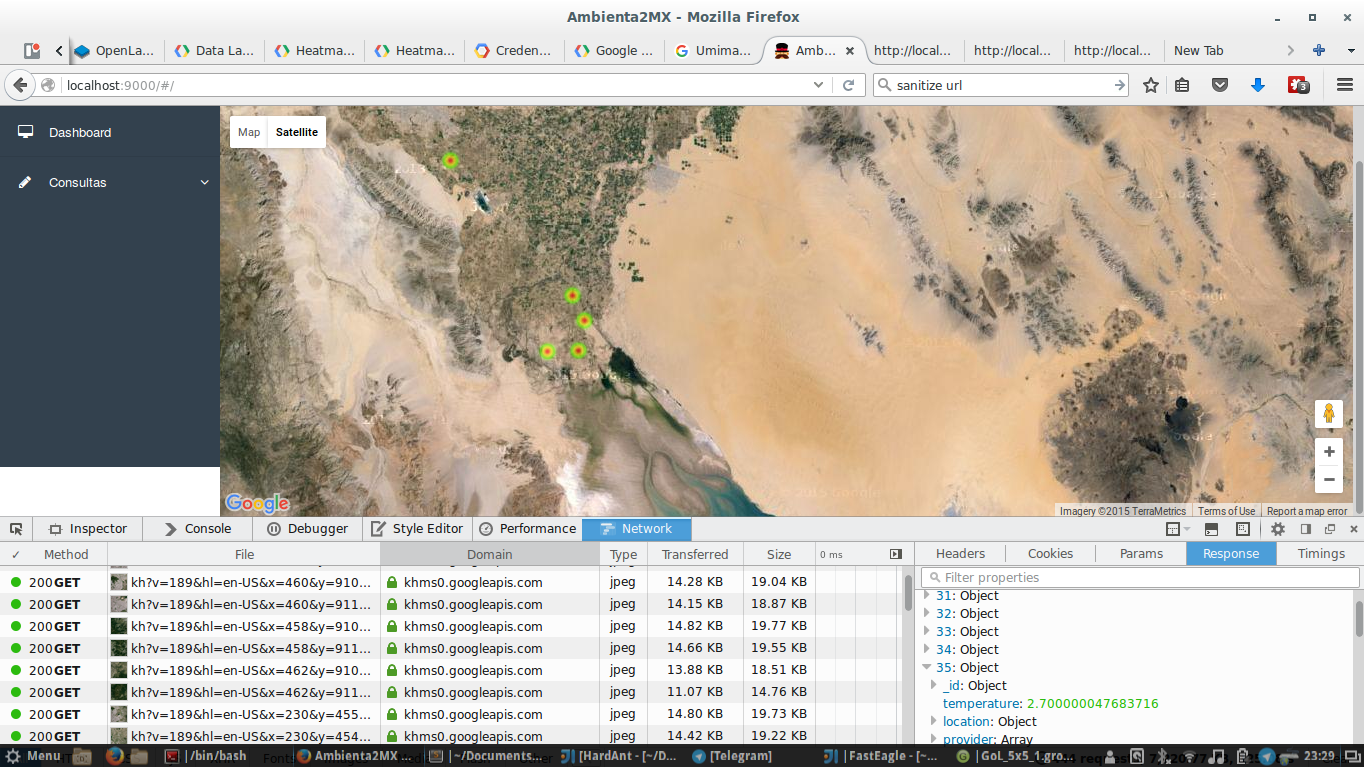
\includegraphics[width=\textwidth]{./images/CapturaFriendlyDolphin}
      \caption{Mapas de Calor, Friendly Dolphin}
    \end{figure}
    \paragraph{Cómo se puede visualizar en la imagen anterior los datos de clima de ciertas regiones del país, en este caso en el área de Baja California, utilizando un concepto llamado HeatMap (Mapa de Calor) que nos permite la transposición de un mapa de Google y los datos climatólogicos recolectados por el sistema de Ambienta2MX. Ésta vista puede ser vista por medio del formulario de busqueda ubicado en la parte superior de las vistas que fueron generadas (véase Figura 8.4).}
    \begin{figure}[b!]
      \centering
        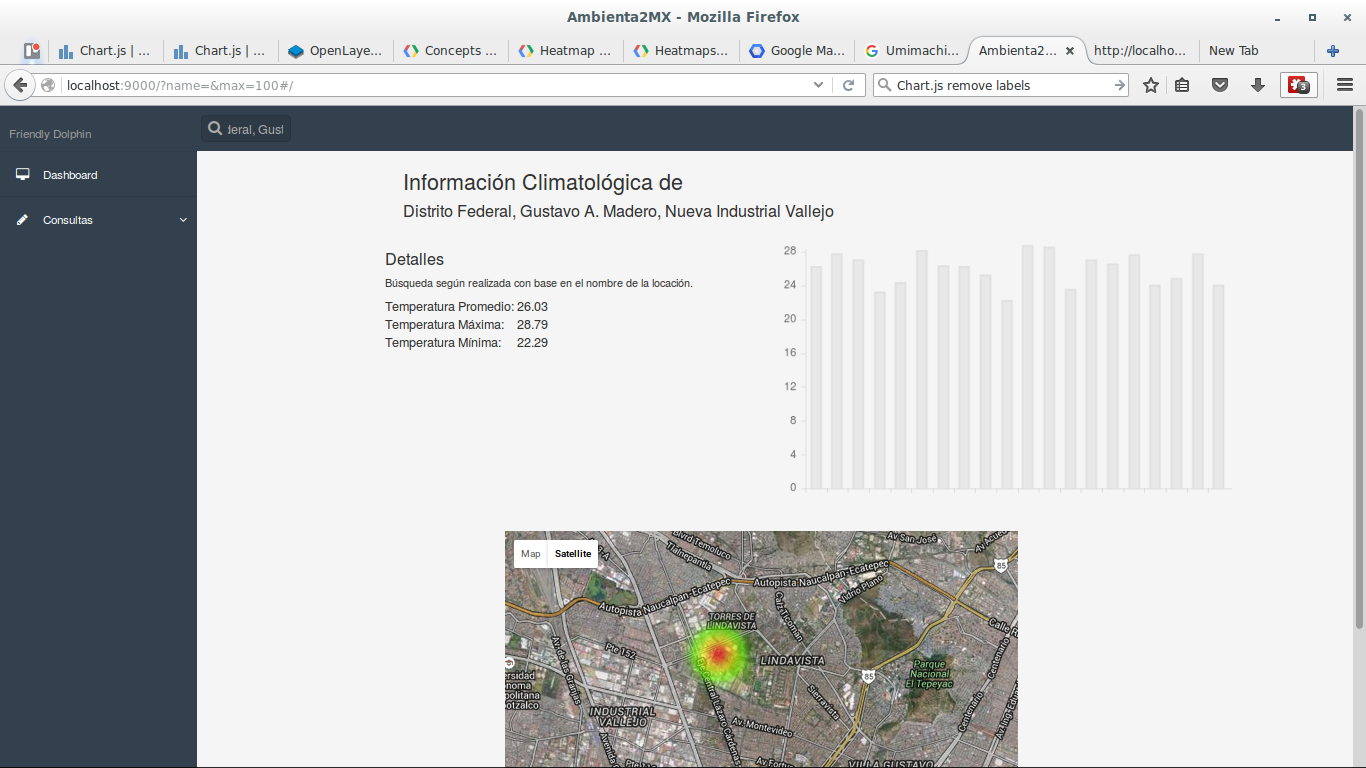
\includegraphics[width=\textwidth]{./images/CapturaFriendlyDolphin2}
      \caption{Tablas e información de clima, Friendly Dolphin}
    \end{figure}
    \paragraph{También puede ser visualizada la información en forma de gráfica de barras, considerando en este caso el área de estudio que es el Distrito Federal, principalmente la parte norte de la capital.}
    \paragraph{El mapa de calor (HeatMap) se traslapa con la vista satelital que nos brinda el servicio de Google Maps. En esta captura se puede apreciar de mejor manera el espectro de temperatura en el área en cuestión, mostrando de un color rojo las áreas con el más alto índice de temperatura y disminuyendo a un color verde en las zonas donde la sensación termica fue menor.}
    \begin{figure}[b!]
      \centering
        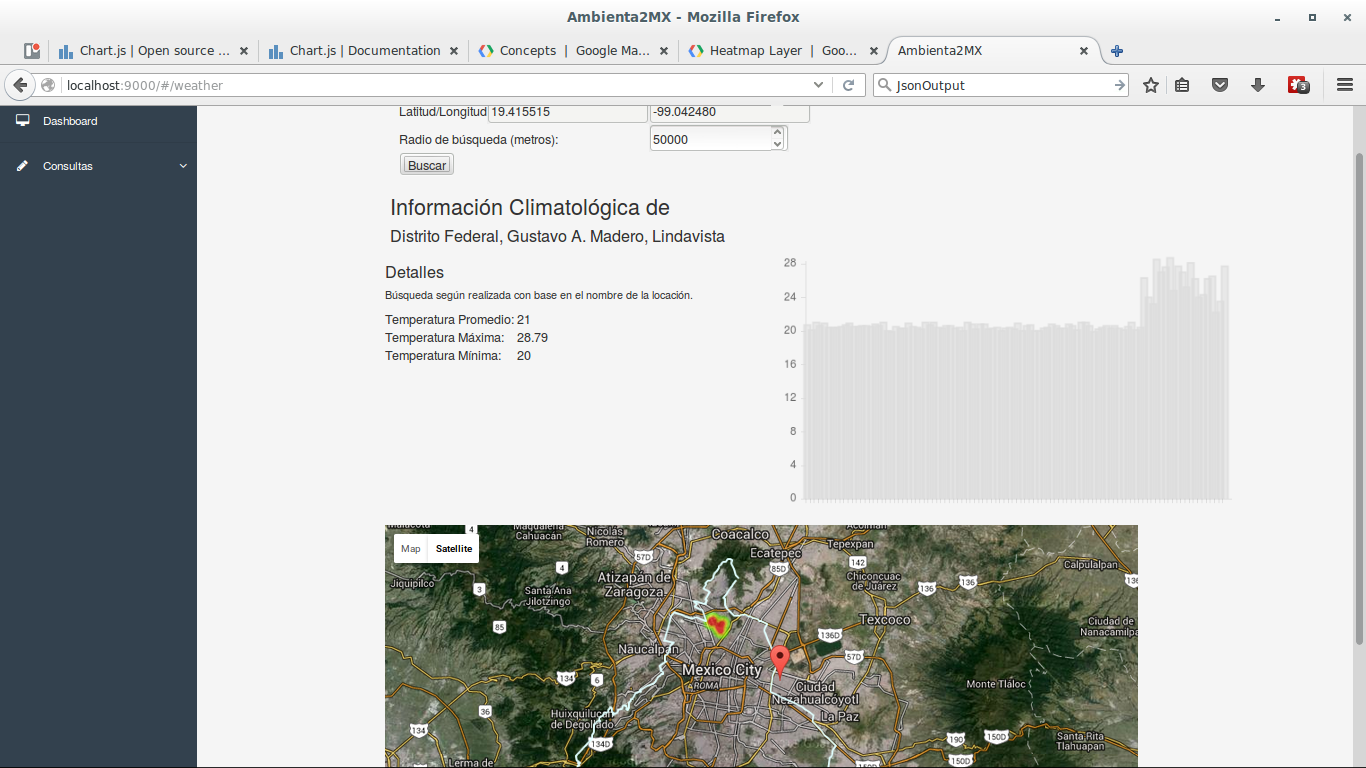
\includegraphics[width=\textwidth]{./images/CapturaFriendlyDolphin3}
      \caption{Tablas e información de clima, Friendly Dolphin}
    \end{figure}
    \paragraph{Cómo puede verse en la siguiente imagen, también se cuenta con una consulta que toma como base un ``Marker'' cólocado por el usuario e índicando el radio de búsqueda en metros. Con ello, el servicio recorrerá las bases de tipo MX para poder encontrar los datos climatológicos o bien de contaminación que cumplen con el criterio de proximidad tomando la información Latitud/Longitud existente en el mapa.}
    \paragraph{Éste tipo de búsqueda resulta util cuando se desea analizar los datos de un área delimitada por un círculo. El ejemplo muestra los datos a 50 kilométros de Ciudad Nezahualcóyotl (Estado de México), coincidiendo con datos de prueba (ubicados en la delegación Gustavo A. Madero), demostrando la funcionalidad de la búsqueda.}
    \paragraph{La información que hace referencia a variables de contaminación ambiental cuenta con pantallas análogas a las mostradas.}
    \paragraph{Las pruebas funcionales fueron ejecutadas utilizando el framework \textbf{iMacros}, a continuación se muestra la rutina que indica la consulta de un lugar y se muestra en la pantalla.}
    \begin{figure}[b!]
      \centering
        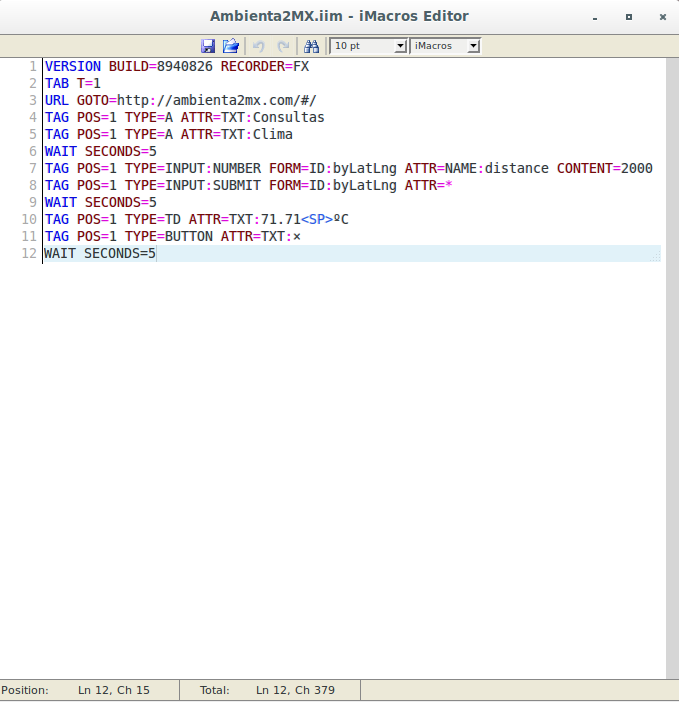
\includegraphics[width=\textwidth]{./images/funcional}
      \caption{Código de prueba funcional}
    \end{figure}